\begin{title}
  Теория кривых
\end{title}

\begin{title}[\Large]
  Параграф 1.1
\end{title}

\begin{title}[\Large]
  Непрерывные, гладкие, регулярные и бирегулярные кривые. Локальное свойство
  регулярной кривой. Касательная и соприкаcающаяся плоскость кривой
\end{title}

\begin{define}[непрерывной кривой]
  Непрерывной кривой называется непрерывное отображение
  $$
  \varphi: [a,b] \to R^3 ~~~ \vec \varphi = \vec \varphi (t), ~~~ t \in [a,b]
  $$
  $\vec \varphi ([a,b]) \subseteq R^3$ называется образом кривой то есть
  множество точек образованных при отображении

  $\vec \varphi (t) = ( x(t), y(t), z(t) )$ вектор функция

  $x = x(t); ~ y = y(t); ~ z = z(t)$ называются координатами функции

  $$
  \left\{
  \begin{array}{c}
    x = x(t) \\
    y = y(t) \\
    z = z(t)
  \end{array}
  \right. ~ \text{параметрическое уравнение кривой}
  $$
\end{define}

\begin{define}[гладкой кривой]
  $\vec \varphi = ( x(t), y(t), z(t) )$ называется гладкая если $\forall k \in N
  ~~~ \exists x^{(k)}(t), y^{(k)}(t), z^{(k)}(t)$
\end{define}

\begin{define}[касательного вектора к кривой]
  Касательный вектор кривой или вектор скорости называется
  $$
  \varphi' (t) = ( x'(t), y'(t), z'(t) ) ~~ \text{или} ~~
  \lim_{ t_{\Delta} \to 0 }
  \frac{ \vec \varphi (t + t_{\Delta}) - \vec \varphi (t) }{t_{\Delta}}
  $$
\end{define}

\begin{define}[особой точки]
  Точка кривой $t_0$ называется особой если $\vec \varphi' (t_0) = \vec 0$
\end{define}

\begin{define}[регулярной кривой]
  Кривая $\vec \varphi = \vec \varphi (t)$ называется регулярной на $[a,b]$ если
  $\forall t \in [a,b] ~~ \vec \varphi' (t) \not = \vec 0$
\end{define}

\begin{define}[инективности и неинективности]
  Инъективно значит каждой точке соответсвует одно значение.

  Неинъективно значит нескольким точкам соответсвует одно значение.
\end{define}

\begin{theorem}
  $\varphi : [a,b] \to R^3$ гладкая кривая, $\exists t_0 \in (a,b)$
  $\vec \varphi' (t_0) \not = 0$ тогда $\exists \varepsilon > 0$
  $\varphi : (t_0 - \varepsilon, t_0 + \varepsilon) \to R^3$ инективно.
\end{theorem}

\begin{define}[касательной прямой регулярной кривой]
  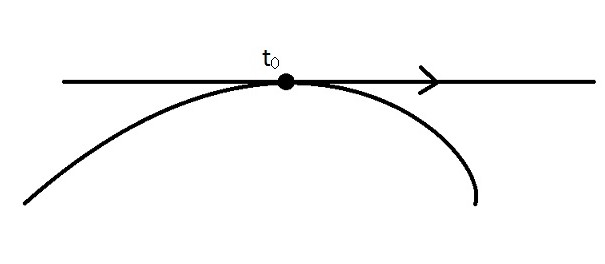
\includegraphics[width = 4.5cm]{tangent}

  $\varphi' (t_0) \not = \vec 0$ тогда касательная прямая
\end{define}

\begin{define}[соприкасающейся плоскости]
  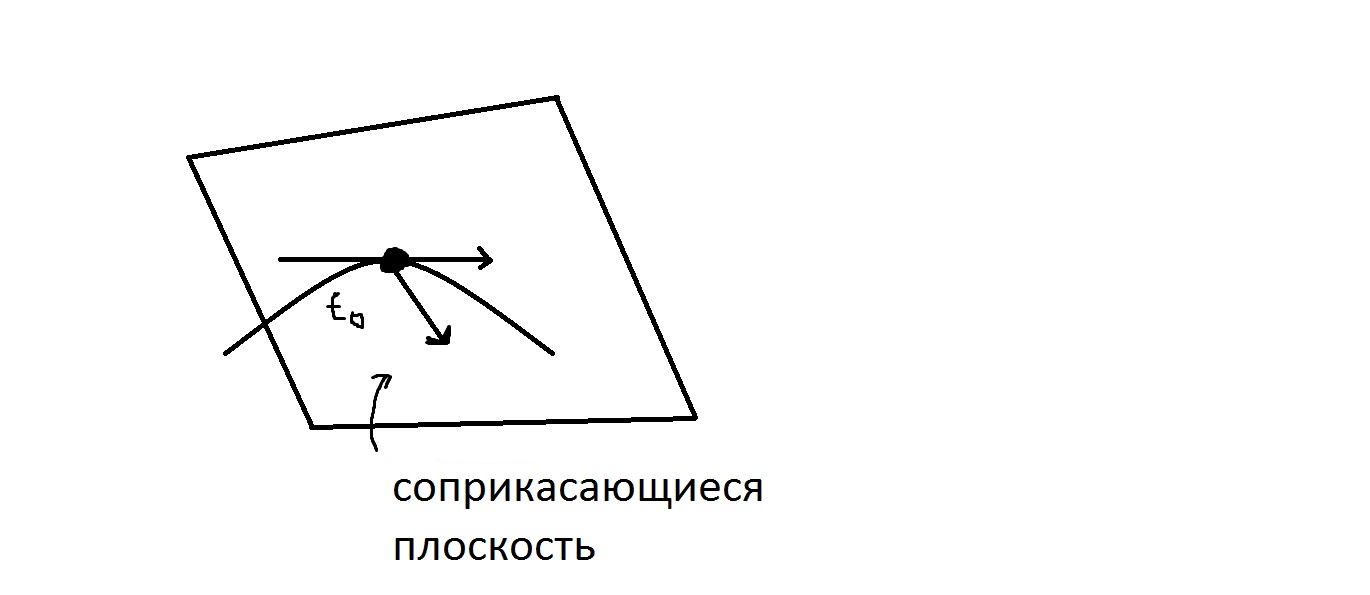
\includegraphics[width = 6cm]{beleg}

  Соприкасающиейся плоскость проходит через точку $t_0$ и пару л.н.з
  векторов $\vec \varphi', \vec \varphi''$.
\end{define}

\begin{define}[точки бирегулярности]
  Точка $t_0$ называется точкой биригулярности, если $\vec \varphi' (t_0),
  \vec \varphi''(t_0)$ линейно независимы (неколинеарны).
\end{define}

\begin{define}[бирегулярности кривой]
  Кривая $\vec \varphi = \vec \varphi(t)$ называется биригулярной если все ее
  точки являются точками бирегулярности

  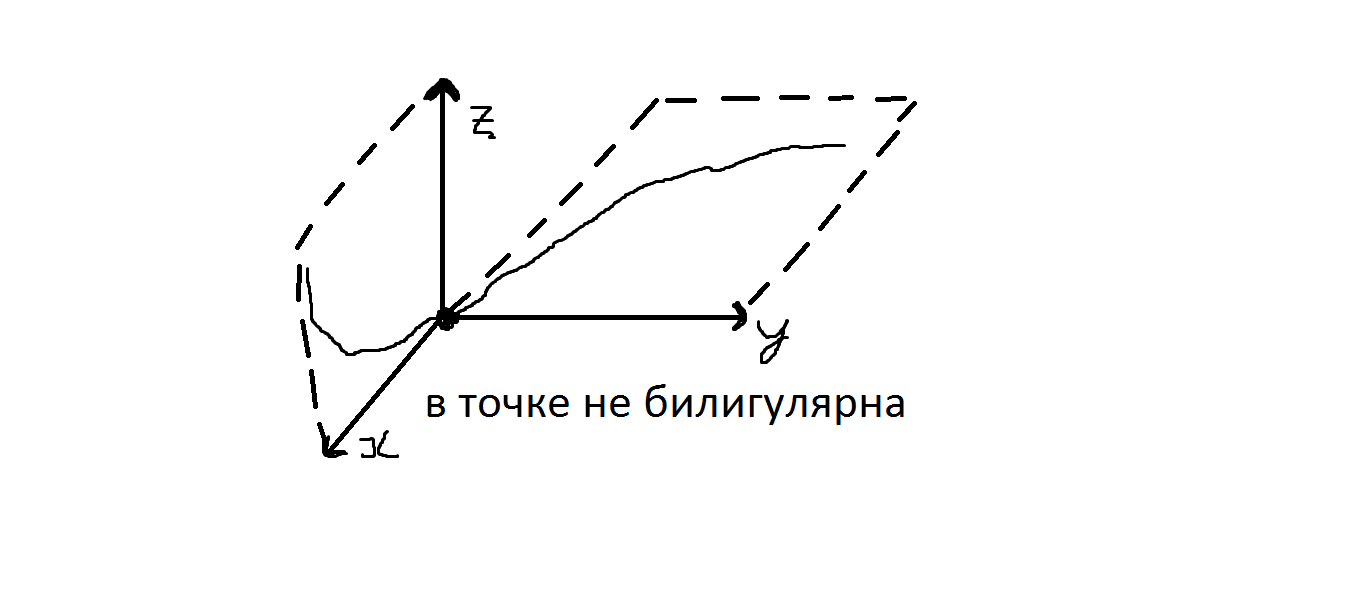
\includegraphics[width = 6cm]{notBeleg}
\end{define}

\begin{title}[\Large]
  Теорема о регулярных кривых на плоскости (в пространстве), заданных неявным
  образом
\end{title}

\begin{theorem}
  $F(x, y) = 0$ гладкая $\exists (x_0, y_0) ~~ F(x_0, y_0) = 0$
  $$
  \grad F(x_0, y_0) = \left( \frac{\partial F(x_0, y_0)}{\partial x},
  \frac{\partial F(x_0, y_0)}{\partial y} \right) \not= \vec 0
  $$
  тогда $\exists (x, y) \in O(x_0, y_0) ~~~ F(x, y) = 0$ является образом
  регулярной кривой.

  В этом случа мы будем говорить что это регулярная кривая задана неявно
  соотношением $F(x, y) = 0$.
\end{theorem}

\begin{theorem}[о неявных функциях]
  Пусть  даны гладкие функции
  $$
  \begin{array}{c}
    F_1 (x_1, x_2, \cdots, x_n, y_1, y_2, \cdots, y_m) \\
    \dots ~~~ \dots ~~~ \dots ~~~ \dots  ~~~ \dots ~~~ \dots \\
    F_m (x_1, x_2, \cdots, x_n, y_1, y_2, \cdots, y_m)
  \end{array}
  $$
  тогда если точка $(x_0, y_0)$ такова что
  $$
  \begin{array}{c}
    F_1(x_0, y_0) = 0 \\
    \ldots ~~~ \ldots \\
    F_m(x_0, y_0) = 0 \\
  \end{array} ~~~~~~
  G(x_0, y_0) = \left|
  \begin{array}{ccc}
    \frac{\partial F_1}{\partial y_1} & \dots &
    \frac{\partial F_1}{\partial y_m} \\

    \dots & \dots & \dots \\

    \frac{\partial F_m}{\partial y_1} & \dots &
    \frac{\partial F_m}{\partial y_m} \\
  \end{array}
  \right|
  \not= 0
  $$
  то $\exists O(x_0, y_0)$ в которой точки улидотворяющие соотношением
  $$
  \left\{
  \begin{array}{c}
    F_1(x, y) = 0 \\
    \dots ~~~ \dots \\
    F_m(x, y) = 0
  \end{array}
  \right. ~~~ \text{задаются} ~~~
  \left\{
  \begin{array}{c}
    y_1 = f_1(x_1, x_2, \cdots, x_n)\\
    \dots ~~~ \dots ~~~ \dots ~~~ \dots \\
    y_m = f_m(x_1, x_2, \cdots, x_n)
  \end{array}
  \right.
  $$
  для некоторых гладких функций $F_1, F_2, \cdots, F_m $
\end{theorem}

\begin{proof}
  По условию в точке $(x_0, y_0)$
  $$
  \grad F(x_0, y_0) = \left( \frac{\partial F(x_0, y_0)}{\partial x},
  \frac{\partial F(x_0, y_0)}{\partial y} \right) \not= \vec 0
  $$
  $\frac{\partial F(x_0, y_0)}{\partial x} \not= 0$ или
  $\frac{\partial F(x_0, y_0)}{\partial y} \not= 0$ $\Rightarrow$
  по теореме о неявной функции $\exists (x, y) \in O(x_0, y_0) ~~~ F(x, y) = 0$
  задается соотношением $y = f(x)$
  то есть состоит из точек вида $(x, f(x))$ $\Rightarrow$ это множество точек
  задается параметрически $(t, f(t))$  $\Rightarrow$
  $(1, f'(x)) \not= \vec 0$ кривая заданная этим уравнением регулярная.
\end{proof}

\begin{block}[Геометрический смысл градиента $F(x,y)$]
  Кривая $F(x, y) = 0$ тогда вектор градиента является нормалью
  (перпендикулярью) касательной кривой и направлен в сторону выпуклости кривой.
\end{block}

\begin{proof}
  По теореме $F(x,y) = 0$ может быть задана параметрической кривой
  $\vec \varphi = (x(t), y(t))$ тогда
  $$
  F(x(t), y(t)) = 0 ~~~
  \frac{dF}{dt} = \frac{\partial F}{\partial x} \frac{dx}{dt} +
  \frac{\partial F}{\partial y} \frac{dy}{dt} =
  (\grad F, \vec \varphi') = 0 ~ \Rightarrow ~ \grad F \perp \vec \varphi'
  $$
\end{proof}